%%%%%%%%%%%%%%%%%%%%%%%%%%%%%%%%%%%%%%%%%
% Professional Mathematical Presentation Template
% 
% This template uses the beamer class with the Madrid theme
% and a custom color scheme for a clean, professional look
% that works well with mathematical content.
%%%%%%%%%%%%%%%%%%%%%%%%%%%%%%%%%%%%%%%%%

\documentclass[aspectratio=169]{beamer} % 16:9 aspect ratio (modern)

% Theme settings
\usetheme{Madrid}
\usecolortheme{default}
\usepackage[dvipsnames]{xcolor}

\definecolor{primcolor}{RGB}{25,50,100} % Dark blue
\setbeamercolor{structure}{fg=primcolor}
\setbeamercolor{frametitle}{bg=primcolor!15, fg=primcolor}
\setbeamercolor{title}{fg=white} % White title text for contrast
\setbeamercolor{subtitle}{fg=white} % White subtitle text
\setbeamercolor{author}{fg=primcolor} % White author text
\setbeamercolor{date}{fg=primcolor} % White date text
\setbeamercolor{institute}{fg=primcolor} % White institute text

% Font settings
\usefonttheme{professionalfonts}
\usefonttheme{serif}

% Package imports
\usepackage{amsmath, amsfonts, amssymb, amsthm} % Math packages
\usepackage{mathtools} % Enhanced math tools
\usepackage{bm} % Bold math symbols
\usepackage{graphicx} % For images
\usepackage{booktabs} % Professional tables
\usepackage{tikz} % For diagrams
\usetikzlibrary{arrows, positioning, matrix, decorations.pathreplacing}

% Use beamer's theorem styles
\setbeamertemplate{theorem}[ams style]
\setbeamertemplate{theorems}[numbered]


% Remove navigation symbols
\setbeamertemplate{navigation symbols}{}

% Custom footer
\setbeamertemplate{footline}{
  \leavevmode%
  \hbox{%
  \begin{beamercolorbox}[wd=.333333\paperwidth,ht=2.25ex,dp=1ex,center]{author in head/foot}%
    \usebeamerfont{author in head/foot}\insertshortauthor
  \end{beamercolorbox}%
  \begin{beamercolorbox}[wd=.333333\paperwidth,ht=2.25ex,dp=1ex,center]{title in head/foot}%
    \usebeamerfont{title in head/foot}\insertshorttitle
  \end{beamercolorbox}%
  \begin{beamercolorbox}[wd=.333333\paperwidth,ht=2.25ex,dp=1ex,right]{date in head/foot}%
    \usebeamerfont{date in head/foot}\insertshortdate{}\hspace*{2em}
    \insertframenumber{} / \inserttotalframenumber\hspace*{2ex} 
  \end{beamercolorbox}}%
  \vskip0pt%
}

% Title information
\title[DP2]{Dynamic Programming}
\subtitle{Thomas J. Sargent and John Stachurski}
\author[Longye]{Longye Tian \\ \texttt{longye.tian@anu.edu.au}}
\institute[ANU]{Australian National University\\ School of Economics}
\date{April 2nd, 2025}
\DeclareFontFamily{U}{mathx}{\hyphenchar\font45}
\DeclareFontShape{U}{mathx}{m}{n}{
      <5> <6> <7> <8> <9> <10>
      <10.95> <12> <14.4> <17.28> <20.74> <24.88>
      mathx10
      }{}
\DeclareSymbolFont{mathx}{U}{mathx}{m}{n}
\DeclareMathSymbol{\bigtimes}{1}{mathx}{"91}

\begin{document}

% Title frame
\begin{frame}
  \titlepage
\end{frame}

% Outline frame
\begin{frame}{Outline}
  \begin{enumerate}
      \item Why Job search Problem?
      \item What is Job Search Problem?
      \item Optimality properties
      \item Rearranging the Bellman equation
  \end{enumerate}
\end{frame}

\begin{frame}{Why Job Search Problem?}
    \begin{itemize}
        \item A good starting point for application 
        \item optimal stopping problem - binary choice
        \item Good for illustrating transformations.
    \end{itemize}
\end{frame}


\begin{frame}{Job Search Model}
    \begin{figure}
        \centering
        \includegraphics[width=0.95\linewidth]{Dynamic Programming/DP2/Chapter 4/Section 4.1.1. Job Search/Job Search Model.png}
    \end{figure}
\end{frame}


\begin{frame}{Job Search Problem Set up}
    We let 
    \begin{itemize}
        \item $W_t$ denote the wage offer drawn from some fixed distribution $\varphi$
        \item $(W_t)_{t\ge 0}$ is IID and take values from $W\subset \mathbb{R}_+$, \textcolor{blue}{$W$ is nonempty}.
        \item $\varphi$ has finite mean, so $\int w\varphi(dw)<\infty$
        \item Constant discount factor $\beta\in(0,1)$
        \item $\Sigma$ be the set of Borel measurable policy $\sigma: W\to \{0,1\}$
         \item $L_1(\varphi):= L^1(W,\mathscr{B}, \varphi)$ be all Borel measurable function $f:W\to \mathbb{R}$ with $\int|f|\,d\varphi<\infty$
    \end{itemize}
\end{frame}
\begin{frame}{Detour to measure theory}
$L_1(\varphi):= L_1(W,\mathscr{B}, \varphi)$ be all Borel measurable function $f:W\to \mathbb{R}$ with $\int|f|\,d\varphi<\infty$.\\
\\
\begin{itemize}
    \item $L^1$-norm is
    $$
    \|f\|_1 = \int_W |f|\, d\varphi
    $$
    \item $f$ is an equivalence class of functions that equals to $f$ almost everywhere
    \item The partial order $f\le g$ means that $\varphi(\{f>g\})=0$
\end{itemize}
\end{frame}


\begin{frame}{Detour to measure theory}
$L^1(\varphi):= L^1(W,\mathscr{B}, \varphi)$ be all Borel measurable function $f:W\to \mathbb{R}$ with $\int|f|\,d\varphi<\infty$.\\
\\
\begin{itemize}
    \item $L^1$-norm is
    $$
    \|f\|_1 = \int_W |f|\, d\varphi
    $$
    \item $f$ is an equivalence class of functions that equals to $f$ almost everywhere
    \item The partial order $f\le g$ means that $\varphi(\{f>g\})=0$
\end{itemize}
$$
\implies
$$
$$
\text{$L^1(\varphi)$ is a \textcolor{red}{\textbf{Banach Lattice}}}
$$
\end{frame}

\begin{frame}{Job Search problem}
We introduce the policy operator $v\mapsto T_\sigma v$ via
$$
(T_\sigma v)(w) = \sigma(w) \frac{w}{1-\beta} + (1-\sigma(w))\left[c+\beta\textcolor{blue}{\underbrace{\int v(w')\, \varphi(dw')}_{\text{Dimension Reduction}}}\right]
$$
    
\end{frame}

\begin{frame}{Deep look into the Policy Operator}
        $$
(T_\sigma v)(w) = \sigma(w) \frac{w}{1-\beta} + (1-\sigma(w))\left[c+\beta\textcolor{blue}{\underbrace{\int v(w')\, \varphi(dw')}_{\text{Dimension Reduction}}}\right]
$$
$$
\text{or equivalently, let $e(w):=\frac{w}{1-\beta}$}
$$

\begin{align*}
    T_\sigma v &= \underbrace{[\sigma e+(1-\sigma)c]}_{=:r_\sigma} + \underbrace{(1-\sigma)\beta \mathbb{E}v}_{=:K_\sigma v}\\
    &= r_\sigma + K_\sigma v
\end{align*}
\end{frame}

\begin{frame}{Deeper look into the policy operator}
    \begin{align*}
    \textbf{\textcolor{red}{\textbf{$T_\sigma v &= r_\sigma + K_\sigma v$}}}
\end{align*}
\begin{itemize}
    \item $T_\sigma$ is \textcolor{red}{\textbf{affine}}
    \item $0\le K_\sigma v = (1-\sigma)\beta\mathbb{E}v\le \beta \mathbb{E}v =:Kv$
    \item we have \textcolor{red}{$K_\sigma \le K$ and $\rho(K) = \beta<1$}
\end{itemize}
\end{frame}



\begin{frame}{ADP formulation}
$$
(T_\sigma v)(w) = \sigma(w) \frac{w}{1-\beta} + (1-\sigma(w))\left[c+\beta\textcolor{blue}{\underbrace{\int v(w')\, \varphi(dw')}_{\text{Dimension Reduction}}}\right]
$$

\begin{itemize}
    \item $v\in L^1(\varphi)\implies T_\sigma v\in L^1(\varphi)$
    \item $T_\sigma$ is order preserving self-map on $L^1(\varphi)$
    \item $\Sigma$ is not empty
\end{itemize}
$$
(L^1(\varphi),\mathbb{T}_{JS}), \quad \mathbb{T}_{JS}:=\{T_\sigma: \sigma\in\Sigma\}
$$
is an ADP for the Job Search Problem. 
\end{frame}

\begin{frame}{The ADP $(L^1(\varphi),\mathbb{T}_{JS})$ is well-posed.}
 $$
 (T_\sigma v)(w) = v(w) 
 $$
 $$
\implies
 $$
    $$
\sigma(w) \frac{w}{1-\beta} + (1-\sigma(w))\left[c+\beta\int v(w')\, \varphi(dw')\right] = v(w)
$$

\begin{itemize}
    \item $\sigma(w) = 1 \implies v(w) = \frac{w}{1-\beta} $ well-defined and unique
    \item $\sigma(w) = 0\implies v(w) = c+\beta\int v(w') \, \varphi(dw')$ well-defined and unique
\end{itemize}

\end{frame}

\begin{frame}{The ADP $(L^1(\varphi),\mathbb{T}_{JS})$ is \textcolor{red}{\textbf{regular}}}
$v$-greedy policy (assume accept the offer at indifference)
    $$
    \sigma (w) = \mathbf{1}\left\{\frac{w}{1-\beta}\ge c+\beta\int v(w') \, \varphi(dw') \right\}
    $$
    with policy operator
    $$
    (T_\sigma v)(w) = \max\left\{\frac{w}{1-\beta}, c+\beta\int v(w') \, \varphi(dw')\right\} \textcolor{blue}{\underbrace{= (Tv)(w)}_{\text{greedy}}}
    $$
\end{frame}

\begin{frame}{Construct Bellman operator from definition}
    $Tv = \bigvee_\sigma T_\sigma v$
    \begin{align*}
        (Tv)(w) &= \left(\bigvee_\sigma T_\sigma v\right)(w)\\
        &= \bigvee_\sigma \left(\sigma(w) \frac{w}{1-\beta} + (1-\sigma(w))\left[c+\beta\int v(w')\, \varphi(dw')\right]\right)\\
        &= \max\left\{\frac{w}{1-\beta}, c+\beta\int v(w') \, \varphi(dw')\right\}
    \end{align*}
    
\end{frame}

\begin{frame}{Bounded $W$ $\implies$ use smaller value space}
$$
\sigma(w) \frac{w}{1-\beta} + (1-\sigma(w))\left[c+\beta\int v(w')\, \varphi(dw')\right]
$$
\begin{itemize}
    \item From $L^1(\varphi)$ to \textcolor{blue}{$bmW$} bounded Borel measurable function
    \item From \textcolor{blue}{$bmW$} to \textcolor{ForestGreen}{$bcW$} bounded continuous function
    \item From \textcolor{ForestGreen}{$bcW$} to \textcolor{Lavender}{$ibcW$} increasing bounded continuous function
    \item From \textcolor{Lavender}{$ibcW$} to \textcolor{RedOrange}{$ibcW_+$} nonnegative increasing bounded continuous function
\end{itemize}
\end{frame}



\begin{frame}{Optimality with IID offers}
    \begin{theorem}
        For $(L^1(\varphi),\mathbb{T}_{JS})$,
        \begin{itemize}
            \item the fundamental optimality properties hold
            \item VFI, OPI, HPI all converge.
        \end{itemize}
    \end{theorem}

    \begin{proof}
    Implore Theorem 1.3.9.\\
\end{proof}

\end{frame}


\begin{frame}{Theorem 1.3.9}

    \begin{figure}
        \centering
        \includegraphics[width=0.85\linewidth]{Dynamic Programming//DP2//Chapter 4//Section 4.1.1. Job Search/thm1.3.9.png}
    \end{figure}


\end{frame}

\section{Rearranging the Bellman Equation}
\begin{frame}{Rearranging the Bellman Equation - Continuation Value}
    Given the Bellman equation
    $$
    v(w)  = \max\left\{\frac{w}{1-\beta}, \textcolor{blue}{c+\beta\int v(w') \,\varphi(dw')}\right\}\quad\text{for all $w\in W$}
    $$
    Let 
    $$
    h:=\textcolor{blue}{c+\beta\int v(w') \,\varphi(dw')}
    $$
    be the continuation value. And $h\in \mathbb{R}$.
\end{frame}

\begin{frame}{Continuation value}
We get a one-dimensional nonlinear equation. 
    \begin{align*}
        h &=\textcolor{blue}{c+\beta\int v(w') \,\varphi(dw')}\\
        &= c + \beta \int \max\left\{\frac{w'}{1-\beta}, \textcolor{blue}{c+\beta\int v(w'') \,\varphi(dw'')}\right\}\, \varphi(dw')\\
        &= c+\beta\int \max\left\{\frac{w'}{1-\beta}, h\right\}\, \varphi(dw')
    \end{align*}
\end{frame}

\begin{frame}{Solve the equation by finding a fixed point}
    We introduce
    $$
    g(h) = c+\beta\int \max\left\{\frac{w'}{1-\beta}, h\right\}\, \varphi(dw')
    $$
    and we want to find the fixed point of $g$. Using the following inequality
    $$
    |\alpha\vee x- \alpha \vee y|\le |x-y|
    $$
    we can show that $g$ is a contraction. Hence we can get a unique fixed point. Optimal policy is hence
    $$
    \sigma_\top (w) = \mathbf{1}\{w\ge w_\top\},\quad \text{where $w_\top:= (1-\beta)h_\top$}
    $$
\end{frame}

\begin{frame}{Reduce the search space further}
    Let $f(h):= c+\beta\bar w/(1-\beta) + \beta h$. We can find the fixed point $h^*$ as
    $$
    h^* = c + \frac{\beta}{1-\beta}\int w\,\varphi(dw) + \beta h^*
    $$
    We have 
    \begin{align*}
        g(h^*) & = c+ \beta \int \max\left\{\frac{w'}{1-\beta}, h^*\right\}\,\varphi(dw')\\
        &= c+ \beta\left(\int_{\{w'/(1-\beta)\ge h^*\}}\frac{w'}{1-\beta}\, \varphi(dw') + \int_{\{w'/(1-\beta)\le h^*\}}h^*\, \varphi(dw')\right)\\
        &= c + \frac{\beta}{1-\beta}\int_{\{w/(1-\beta)\ge h^*\}}w\,\varphi(dw) + \beta h^*\varphi(\{w/(1-\beta)\le h^*\})
    \end{align*}
\end{frame}

\begin{frame}{Reduce the search space continued}

$$
 h^* = c + \frac{\beta}{1-\beta}\int w\,\varphi(dw) + \beta h^*
$$

$$
 g(h^*) =c + \frac{\beta}{1-\beta}\int_{\underbrace{\{w/(1-\beta)\ge h^*\}}_{\varphi(\cdot)\le1}}w\,\varphi(dw) + \beta h^*\underbrace{\varphi(\{w/(1-\beta)\le h^*\})}_{\le1}\le h^*
$$
Hence, $g$ maps $h^*$ down.\\
\\
$g$ is a contraction $\implies$ globally stable $\implies$ strongly order stable $\implies$ $g$ is a self-map on $[0, h^*]$.
\end{frame}

\begin{frame}{Parametric Monotonicity}
    \begin{itemize}
        \item parameters play a key role in dynamics
        \item Is the solution robust to parameter change?
        \item  How does the solution vary with parameters?
        \item Useful to robustness check
        \item useful to policy design
    \end{itemize}
\end{frame}

\begin{frame}{Parametric Monotonicity}
        Given the Bellman equation
    $$
    v(w)  = \max\left\{\frac{w}{1-\beta}, c+\beta\int v(w') \,\varphi(dw')\right\}\quad\text{for all $w\in W$}
    $$
    How does changes in 
    \begin{itemize}
        \item unemployment compensation $c$
        \item discount factor $\beta$
        \item distribution $\varphi$
    \end{itemize}
    change the reservation wage $w_\top = (1-\beta) (c+\beta\int v_\top(w')\, \varphi(dw'))$.
\end{frame}

\begin{frame}{Proposition A.5.18}
Let $V$ be a pospace and $S,T$ be two self-map on $V$ ordered pointwise, i.e.,
$$
S\precsim T\iff Sv\precsim Tv\quad \text{for all $v\in V$}
$$
If $S\precsim T$, $T$ is \textcolor{blue}{order preserving and globally stable} on $V$, then its unique fixed points dominates any fixed point of $S$.
\begin{proof}
   $$
   v_S = Sv_S\precsim Tv_S\implies v_S\precsim v_T
   $$
   by (strongly) order stability from global stability + order preserving.
\end{proof}
    
\end{frame}

\begin{frame}{Unemployment Compensation}
    We have for $c_1\le c_2$
    $$
    g_1(h) = c_1 + \beta \int \max\left\{\frac{w'}{1-\beta}, h\right\}\,\varphi(dw')\le c_2 + \beta \int \max\left\{\frac{w'}{1-\beta}, h\right\}\,\varphi(dw') = g_2(h)
    $$
\begin{itemize}
    \item By \textcolor{blue}{PropA518}, $h^1_\top \le h^2_\top$.
    \item By $w_\top = (1-\beta)h_\top$, $w^1_\top\le w^2_\top$
\end{itemize}
Higher unemployment compensation, higher reservation wage.
\end{frame}

\begin{frame}{Higher unemployment compensation, wait longer on average}
Let $\tau$ be the first passage time to employment, i.e.,
$$
\tau:= \inf\{t\ge 0: \sigma_\top (W_t) = 1\} = \inf\{t\ge 0: W_t\ge w_\top\}
$$
\textbf{Remark:} Here $\tau$ is a random variable with sample space $\Omega = W^\mathbb{N}$. We have
\begin{align*}
    \mathbb{E}\tau  &= 0\cdot \mathbb{P}(W_0\ge w_\top) + 1\cdot \mathbb{P}(W_1\ge w_\top
    |W_0< w_\top)+ 2\cdot \mathbb{P}(W_2\ge w_\top|W_0,W_1<w_\top)+\cdots\\
    &= 0\cdot p + 1\cdot p(1-p) + 2\cdot p(1-p)^2 + \cdots\\
    &= \sum_{i=1}^\infty ip(1-p)^i\tag{mean of Geometric distribution}\\
    &=\frac{1-p}{p}
\end{align*}
\end{frame}

\begin{frame}{Higher unemployment compensation, wait longer on average}
    We have $c_1\le c_2\implies w_\top^1\le w_\top^2$, this implies
    $$
    p_1 = \mathbb{P}(W_i\ge w^1_\top)\ge \mathbb{P}(W_i\ge w_\top^2) = p_2
    $$
    $$
    p_1\ge p_2\implies\mathbb{E}\tau|c=c_1 = \frac{1-p_1}{p_1} \le  \frac{1-p_2}{p_2} = \mathbb{E}\tau|c=c_2
    $$
\end{frame}

\begin{frame}{Increase in discount factor}
From 
$$
h_\top = c+\beta\int\max\left\{\frac{w'}{1-\beta}, h_\top\right\}\, \varphi(dw')
$$
We use $w_\top = (1-\beta)h_\top$ get
$$
w_\top  = c(1-\beta)  + \beta\int\max\{w', w_\top\}\,\varphi(dw')
$$
We define the following function (\textcolor{blue}{order-preserving and contraction}):
$$
f(w) =  c(1-\beta)  + \beta\int\max\{w', w\}\,\varphi(dw')
$$
And $w_\top$ is the unique fixed point. 
\end{frame}

\begin{frame}{Increase in discount factor}
We can take partial derivative of $f$ with respect to $\beta$
$$
\frac{\partial f(w)}{\partial \beta} = -c+\int\max\{w',w\}\,\varphi(dw')
$$
Hence, when 
$$
c\le \int w'\,\varphi(dw') \le \int\max\{w',w\}\,d(w')\quad \text{for all $w\in W$}
$$
We have for $\beta_1\le\beta_2$
$$
\textcolor{blue}{f(w;\beta_1)\le f(w;\beta_2)\quad \text{for all $w\in W$}}
$$
By \textcolor{blue}{PropA518}, we have $w_\top^1\le w_\top^2$.
\end{frame}



\begin{frame}{Changes in distribution}
If $\psi$ first order stochastically dominates $\varphi$, then $w_\top^\varphi\le w_\top^\psi$.
\begin{definition}
    Let $ibX$ be the increasing bounded real-value functions on $X$. We say that $\nu$ first order stochastically dominates $\mu$ and write $\mu\precsim_F \nu$ if 
    $$
    \int u(x)\,\mu(dx)\le \int u(x)\,\nu(dx)\quad\text{for every $u\in ibX$}
    $$
\end{definition}
\begin{proof}
     We have for $c_1\le c_2$
    $$
    g_\varphi(h) = c + \beta \int \max\left\{\frac{w'}{1-\beta}, h\right\}\,\varphi(dw')\le c+ \beta \int \max\left\{\frac{w'}{1-\beta}, h\right\}\,\psi(dw') = g_\psi(h)
    $$
\end{proof}
    
\end{frame}


\begin{frame}{Mean-preserving spread}
    We also concern with how behavior changes when decisions become riskier. We introduce the notion of \textbf{mean-preserving spread}. For a given distribution $\varphi$, we say that $\psi$ is a mean-preserving spread of $\varphi$ if there exists a pair of random variable $(Y,Z)$ such that
    $$
    \mathbb{E}[Z|Y] = 0,\quad Y=^d \varphi, \quad Y+Z=^d\psi 
    $$
\end{frame}

\begin{frame}{In this question}
We know that
$$
W =^d \varphi
$$
Let $\psi$ be a mean-preserving spread of $\varphi$. Then there exists a pair of random variable $(W,Z)$ such that
$$
\mathbb{E}[Z|W] = 0,\quad W=^d\varphi, \quad W+Z=^d\psi
$$
This implies
\begin{align*}
    \int\max\{w',w\}\,\psi(dw') &= \mathbb{E}[\max\{W+Z, w\}]= \mathbb{E}\bigg[\mathbb{E}[\max\{W+Z, w\}|W]\bigg]\tag{LIE}\\
    &\ge \mathbb{E}\bigg[\max\{\mathbb{E}[W+Z|W],w\}\bigg]\tag{Cond. Jensen}\\
    &= \mathbb{E}\bigg[\max\{W,w\}\bigg]\tag{Linearity}\\
    &= \int\max\{w',w\}\,\varphi(dw')
\end{align*}
\end{frame}

\section{Job Search with Correlated Wage Draws}
\begin{frame}{Deep look into the Policy Operator}
        $$
(T_\sigma v)(w) = \sigma(w) \frac{w}{1-\beta} + (1-\sigma(w))\left[c+\beta\textcolor{blue}{\underbrace{\int v(w')\, \varphi(dw')}_{\text{Dimension Reduction}}}\right]
$$
$$
\text{or equivalently, let $e(w):=\frac{w}{1-\beta}$}
$$

\begin{align*}
    T_\sigma v &= \underbrace{[\sigma e+(1-\sigma)c]}_{=:r_\sigma} + \underbrace{(1-\sigma)\beta \mathbb{E}v}_{=:K_\sigma v}\\
    &= r_\sigma + K_\sigma v
\end{align*}
\end{frame}

\begin{frame}{Comparison}
\textbf{For IID draws}
\begin{align*}
    T_\sigma v &= \underbrace{[\sigma e+(1-\sigma)c]}_{=:r_\sigma} + \textcolor{blue}{\underbrace{(1-\sigma)\beta \mathbb{E}v}_{=:K_\sigma v}}\\
    &= r_\sigma + \textcolor{blue}{K_\sigma v}
\end{align*}

\textbf{For Correlated wage draws}
\begin{align*}
    T_\sigma v &= \underbrace{[\sigma e+(1-\sigma)c]}_{=:r_\sigma} + \textcolor{blue}{\underbrace{(1-\sigma)\beta P}_{:=\beta P_\sigma}v}\\
    &= r_\sigma +\textcolor{blue}{\beta P_\sigma v}
\end{align*}
We assume $(W_t)$ is $P$-Markov with stationary distribution $\varphi$, $\int w\,\varphi(dw)<\infty$
\end{frame}

\begin{frame}{Optimality}
\begin{itemize}
    \item Value space is also Banach lattice
    \item $T_\sigma$ also order-preserving self-map
    \item Similar proof for well-posedness and regularity
    \item Similar affine and bounded by $\beta P$
    \item Same optimality results
\end{itemize}
    
\end{frame}

\begin{frame}{Difference}
\begin{itemize}
    \item wage draws are not iid anymore
    \item cannot reduce dimensions as before
\end{itemize}
    
\end{frame}
\begin{frame}{Reducing the value space}
    Let $\bar v:= (I-\beta P)^{-1}(e+c)$ and $V:= \{v\in L_1(\varphi): 0\le v\le \bar v\}$. Previously we have shown
    $$
    v_\sigma  = (I-\beta P_\sigma)^{-1}r_\sigma
    $$
    where $P_\sigma v =   (1-\sigma)P v \precsim Pv $, $r_\sigma  = \sigma e +(1-\sigma)c\precsim e+c$.\\
    \\
    
    Hence, we have
    $$
    v_\sigma \le \bar v
    $$
    By global stability and order preserving, $T_\sigma V\subset V$, i.e., self-map on $V$.
\end{frame}

\begin{frame}{Optimality on the reduced value space}
    \begin{figure}
        \centering
        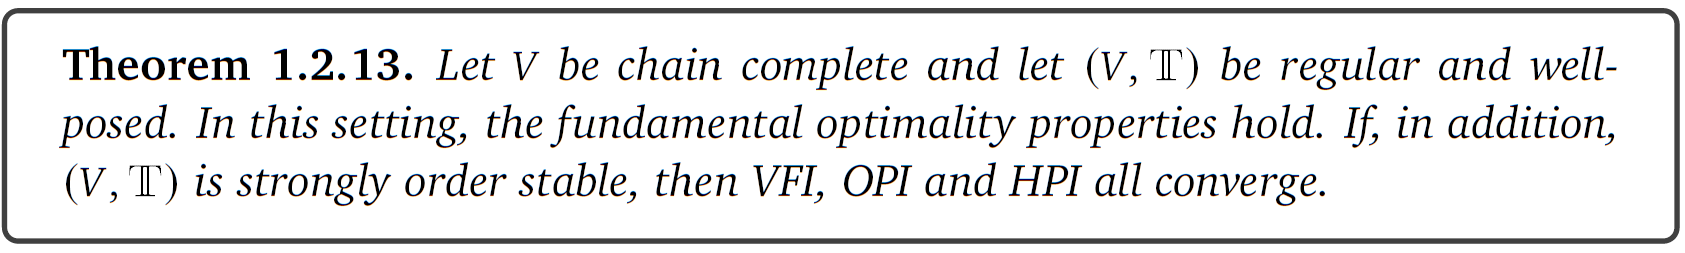
\includegraphics[width=1\linewidth]{Dynamic Programming/DP2/Chapter 4/Section 4.1.1. Job Search/thm 1.2.13.png}
        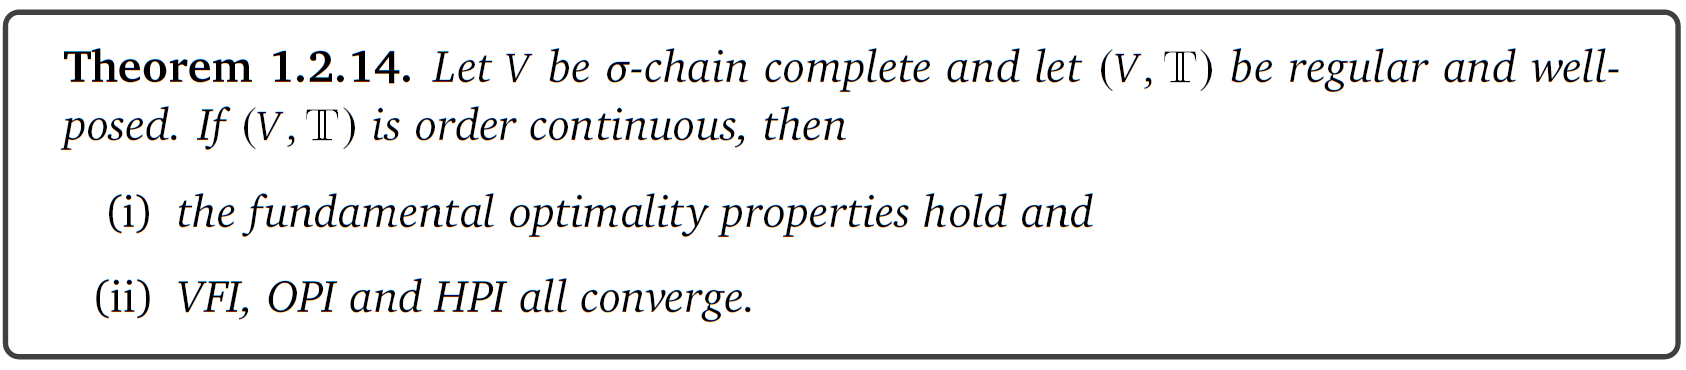
\includegraphics[width=1\linewidth]{Dynamic Programming/DP2/Chapter 4/Section 4.1.1. Job Search/thm1.2.14.png}
    \end{figure}
\end{frame}

\end{document}
